\documentclass[../summary.tex]{subfiles}

\begin{document}
\section{Raw materials and circular economy}
\subsection{Introduction}	
\subsubsection{What are resources}
	
Our prosperity relies on easy access to abundant raw materials, with global demand exceeding 100 billion tonnes annually and predicted to double by 2060. Raw materials, substances or resources processed for product creation, are sourced from the earth's crust, nature, and recycled waste in the economy or technosphere. \\
\\
Examples of raw materials from the lithosphere or earth crust are fossil oil and gas, iron ore, bauxite as raw material for aluminium, minerals such as sand or marble, lithium brines, and so on. Metals are often found in ores with varying concentrations, and their distribution is uneven globally. Biomass, derived from nature, includes plant-based and animal-derived materials. Secondary raw materials, extracted from recycled waste, vary in extraction rates, e.g., lead at 70\%, while lithium remains below 1\%. Despite recycling efforts, 88 to 94\% of materials in new products still come from primary resources. \\
\\
Raw material sources span the litho-, bio-, and technosphere. The industrial metabolism concept likens the economy's material processes to the human body's metabolism, providing insight into material management, waste, and emissions for sustainable improvements.

\subsubsection{Case: Electric car}

The ongoing effort to combat climate change includes a significant focus on the energy transition, with a key aspect being the widespread adoption of electric vehicles (EVs). The transition is evident in the rapid increase in EV sales, accounting for 14\% of new car sales in 2022, up from 9\% in 2021 and 5\% in 2020. Figure \ref{fig:electriccarsales} depicts a substantial rise in electric car sales, reaching an estimated 14 million in 2023, with 8 million sold in China.

\begin{figure}[H]
	\centering
	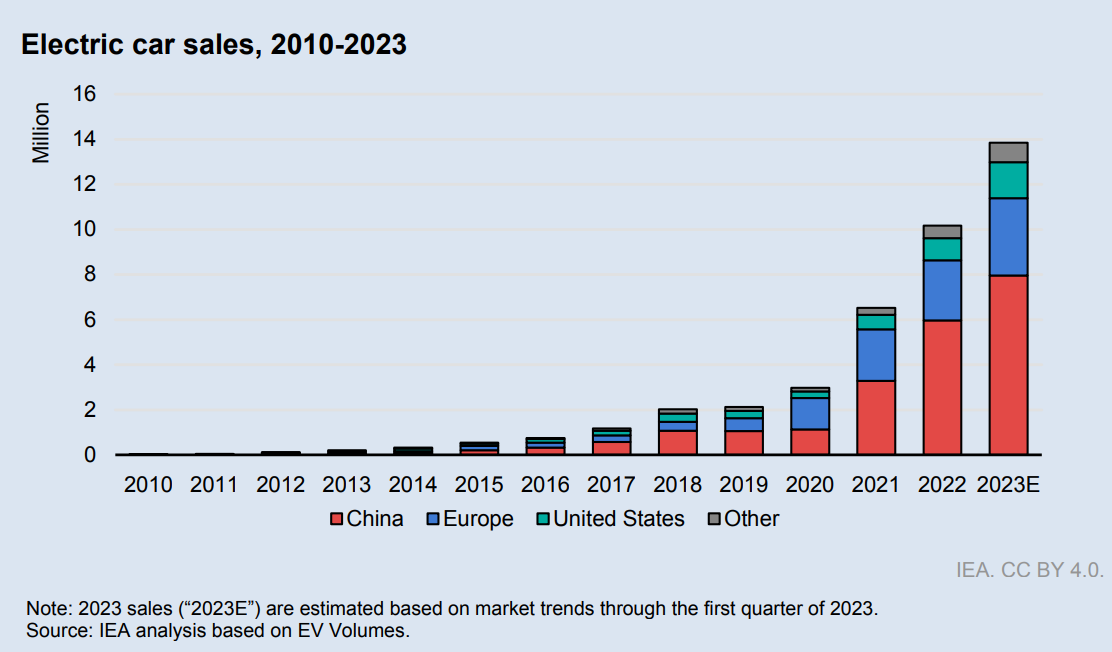
\includegraphics[width=0.7\linewidth]{../images/Electric_car_sales}
	\caption{Electric car sales between 2010 and 2023}
	\label{fig:electriccarsales}
\end{figure}
\ \\
The shift to EVs brings about a change in the materials used, replacing combustion engines with catalysts containing Pt, Pd, and Rh with electric motors requiring copper and neodymium magnets (NdFeB). Power is supplied by Li-ion batteries, raising concerns about the availability of materials to meet the growing demand. Questions arise regarding the duration of lithium availability for Li-ion batteries and the overall environmental impact of EVs compared to traditional combustion engine vehicles. Additionally, considerations about battery recycling and recyclability play a crucial role in evaluating the sustainability of electric vehicles.

\subsection{Material demand}
\subsubsection{trends in material demand}

Over the past five decades, global demand for materials has surged, more than tripling, outpacing both population and GDP growth. While the world's population doubled during this period, the \textbf{gross domestic product} (GDP) quadrupled. The implications of this growth raise questions about the future trajectory of our material needs over the next 10, 20, or 100 years. To forecast this trajectory, an analysis of the driving forces behind the evolution of global material demand is crucial.\\
\\
Three primary factors propel global material demand: population, affluence (which represents the average level of wealth per person, measured by GDP per capita), and technology (material intensity per dollar of GDP). While population growth continues, its significance in driving material demand is diminishing due to declining growth rates. Affluence, reflecting individual wealth, has seen a consistent growth rate when adjusted for inflation and cost of living, leading to a stable projection for the foreseeable future.\\
\\
The most intricate factor, technology, involves examining the material efficiency of the economy. Comparisons between GDP per person and material footprint per person across countries reveal a trend – larger GDP correlates with a larger material footprint, but the relationship is not strictly linear. This observation holds true over the years, suggesting a pattern in global evolution.\\
\\
In industrialized nations, a notable trend emerges – a relative decoupling of economic growth and material demand growth. While the absolute material footprint increases, the relative footprint per dollar of GDP decreases. This pattern contrasts with countries undergoing industrialization, such as China in the past 30 years, where material demand grew faster than GDP due to intense infrastructure development.\

\begin{figure}[H]
	\centering
	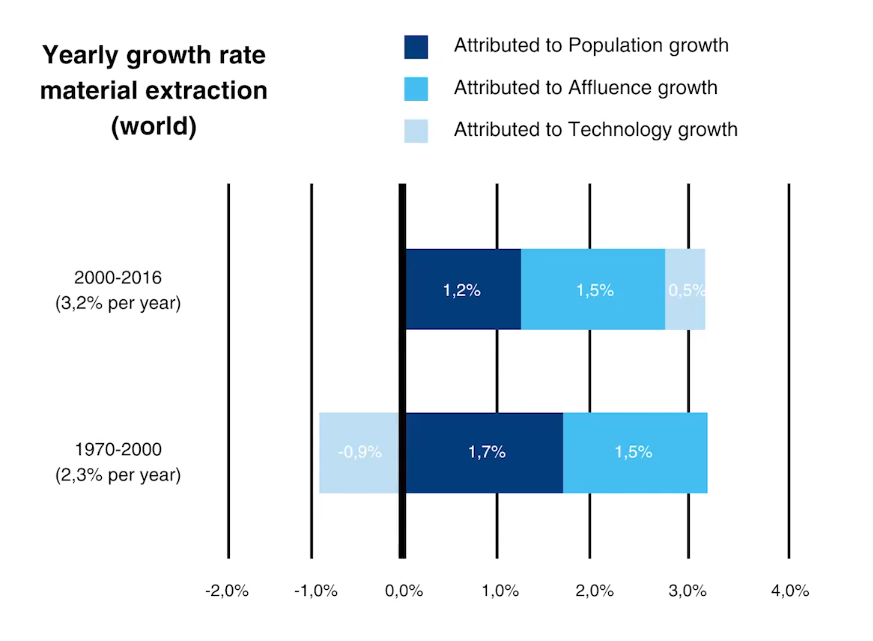
\includegraphics[width=0.7\linewidth]{../images/material_demand_growth_rates}
	\caption{Material demand growth rates throughout the past 50 years}
	\label{fig:materialdemandgrowthrates}
\end{figure}
\ \\
Looking ahead, the future trajectory involves anticipating the dynamics of these three factors. Population growth will continue but at a slower pace. Affluence will persist in its growth to ensure equal opportunities globally. The technology factor, representing material intensity, is expected to vary across countries. China, a significant purchaser of materials, is forecasted to enter a less material-intensive phase, while countries like India and many African nations may undergo material-intensive development phases.\\
\\\\
The Organisation for Economic Co-operation and Development (OECD) foresees a doubling of worldwide material demand by 2060, indicating further growth. However, this growth will not be uniform across all material types. Materials crucial for the energy transition, such as lithium, are expected to experience much higher growth rates. For instance, demand for lithium in 2050 is projected to be 20 times higher than today, emphasizing the changing landscape of material needs in the context of evolving technologies and global priorities.

\subsubsection{Case: Electric car}

The shift towards electrical mobility requires a lot of materials that where not very much used before, such as Lithium, and an substantial increase in demand of some commodities, such as Nickel or Copper. Figure \ref{fig:Lithium} and \ref{fig:Nickel} underneath show the forecasted demand for the coming decades of lithium and nickel, in the case of the STEPS and SDS IEA scenarios.

\begin{figure}[H]
	\centering
	\begin{subfigure}{.5\textwidth}
		\centering
		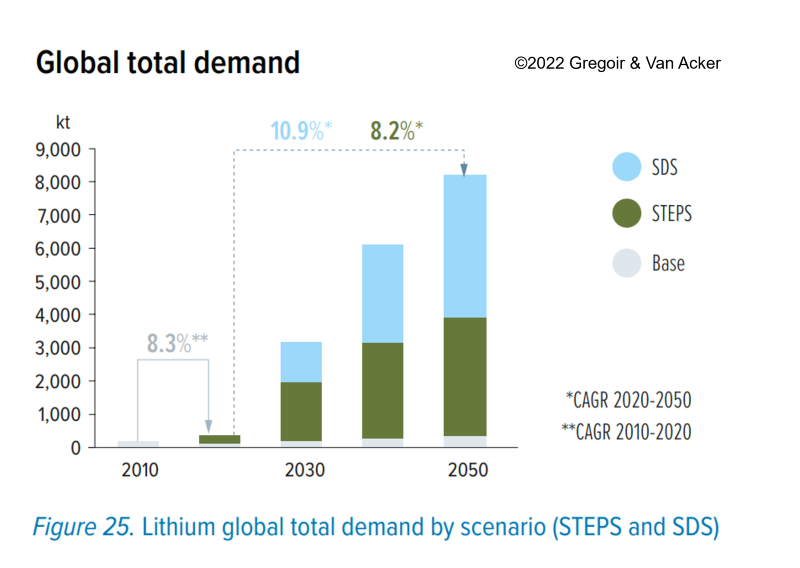
\includegraphics[width=1\linewidth]{../images/Global_lithium_demand_STEPS_SDS}
		\caption{Lithium}
		\label{fig:Lithium}
	\end{subfigure}%
	\begin{subfigure}{.5\textwidth}
		\centering
		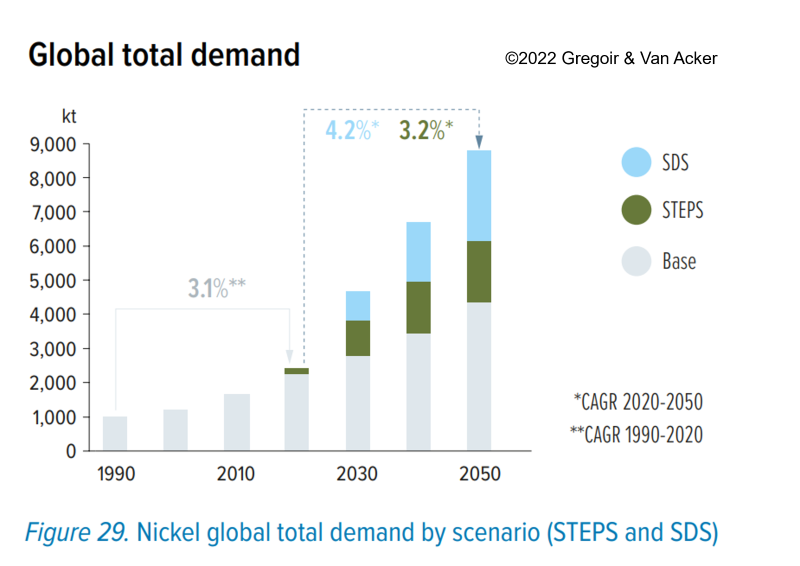
\includegraphics[width=1\linewidth]{../images/Global_nickel_demand_STEPS_SDS}
		\caption{Nickel}
		\label{fig:Nickel}
	\end{subfigure}
	\caption{Global total demand by STEPS  and SDS scenarios}
	\label{fig:Global total demand}
\end{figure}
\ \\
Two scenarios as put forward by the International Energy Agency are considered in these figures:\\
\\
\textbf{The Stated Policies Scenario (STEPS) }reflects current policy settings based on a sector-by-sector assessment of the specific policies that are in place, as well as those that have been announced by governments around the world. It provides an indication of where today’s policy measures and plans lead the energy sector.\\
\\
\textbf{The Sustainable Development Scenario (SDS) }charts a pathway that meets in full the world’s goals to tackle climate change in line with the Paris Agreement while meeting universal energy access and significantly reducing air pollution. In this scenario, all current net zero pledges are achieved in full and there are extensive efforts to realize near-term emissions reductions; advanced economies reach net zero emissions by 2050, China around 2060, and all other countries by 2070 at the latest.

\end{document}